\documentclass{article}
\usepackage[utf8]{inputenc}
\usepackage{xcolor}
\usepackage{graphicx}
\usepackage{float}
\usepackage{minted}
\usepackage{circuitikz}
\usepackage{tikz}
\usetikzlibrary{shapes, arrows, calc, positioning, circuits.logic.US, circuits.logic.IEC}
\usepackage{geometry}
\geometry{a4paper, margin=1in}
\usepackage{hyperref}
\usemintedstyle{trac}

\usepackage{fancyhdr}
\pagestyle{fancy}
\fancyhf{}
\renewcommand{\headrulewidth}{0pt}
\fancyfoot[C]{\small 010153101 Digital Circuit and Microprocessor Fundamental \\ Semester 2/2025}
\fancyfoot[R]{\thepage}

\fancypagestyle{plain}{%
  \fancyhf{}%
  \fancyfoot[C]{\small 010153101 Digital Circuit and Microprocessor Fundamental \\ Semester 2/2025}%
  \fancyfoot[R]{\thepage}%
  \renewcommand{\headrulewidth}{0pt}%
}

\title{Laboratory Exercise 7 - Week 2 \\ Applications of Counters}
\author{}
\date{}

\begin{document}

\maketitle

This week focuses on applications of counters, including timing generation and controlling display sequences.

\setcounter{figure}{3}

\section*{Part IV}

Design and implement a circuit that successively flashes digits 0 through 9 on the 7-segment display HEX0. Each digit should be displayed for about one second. Use a counter to determine the one-second intervals. The counter should be incremented by the 50-MHz clock signal provided on the DE0-CV board. For the output, you can use the 7-segment decoder from previous exercises.

\begin{figure}[H]
    \centering
    \resizebox{\textwidth}{!}{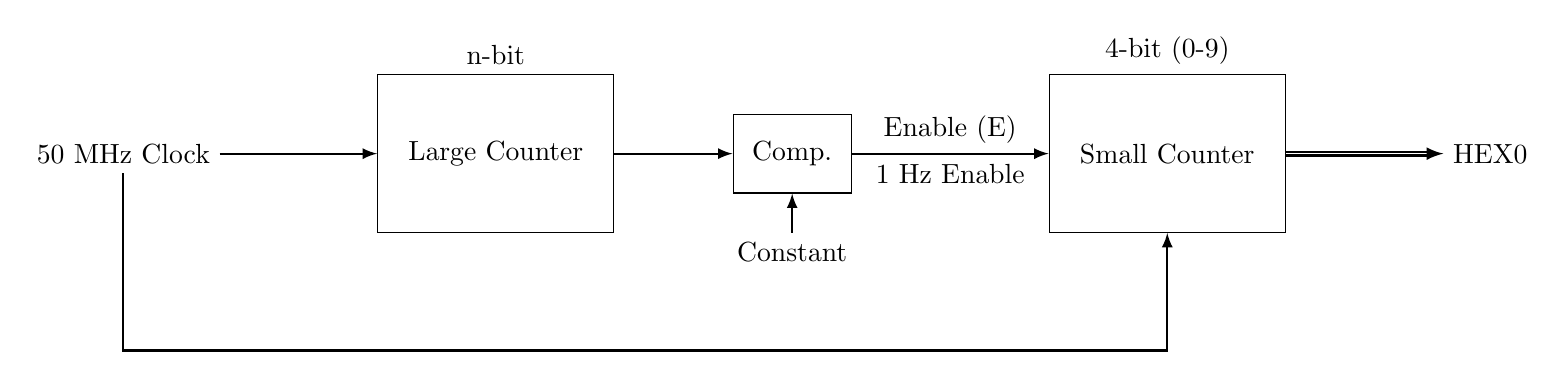
\begin{tikzpicture}[auto, node distance=2cm,>=latex]
    % Large Counter
    \node [draw, minimum width=3cm, minimum height=2cm] (large_cnt) {Large Counter};
    \node [anchor=south] at (large_cnt.north) {n-bit};
    
    % Inputs
    \node [left=of large_cnt] (clk) {50 MHz Clock};
    \draw [->, thick] (clk) -- (large_cnt.west);
    
    % Comparator
    \node [draw, minimum width=1.5cm, minimum height=1cm, right=1.5cm of large_cnt] (cmp) {Comp.};
    
    % Constant Input
    \node [below=0.5cm of cmp] (const) {Constant};
    \draw [->, thick] (const) -- (cmp.south);
    
    % Small Counter
    \node [draw, minimum width=3cm, minimum height=2cm, right=2.5cm of cmp] (small_cnt) {Small Counter};
    \node [anchor=south] at (small_cnt.north) {4-bit (0-9)};
    
    % Connections
    \draw [->, thick] (large_cnt.east) -- (cmp.west);
    \draw [->, thick] (cmp.east) -- (small_cnt.west) node[midway, above] {Enable (E)} node[midway, below] {1 Hz Enable};
    
    % Clock for Small Counter (Same 50MHz)
    % The diagram in Lab 4 might imply the small counter is enabled by the large one but clocked by the same clock
    \draw [->, thick] (clk) -- ++(0, -2.5) -| (small_cnt.south);
    
    % Output
    \node [right=of small_cnt] (hex) {HEX0};
    \draw [->, thick, double] (small_cnt.east) -- (hex);

\end{tikzpicture}
}
    \caption{Making a slow counter to drive a display.}
    \label{fig:slow_counter}
\end{figure}

Do not derive any other clock signals in your design—make sure that all flip-flops in your circuit are clocked directly by the 50-MHz clock signal. A partial design of the required circuit is shown in Figure \ref{fig:slow_counter}. The figure shows how a large bit-width counter can be used to produce an enable signal for a smaller counter.

For reference, an example of a counter specified using a generic parameter \texttt{n} is shown in Figure \ref{fig:generic_counter}.

\begin{figure}[H]
    \centering
    \begin{minted}[frame=single, fontsize=\small, linenos]{vhdl}
LIBRARY ieee;
USE ieee.std_logic_1164.all;
USE ieee.numeric_std.all;

ENTITY counter IS
    GENERIC ( n : INTEGER := 4 );
    PORT ( Clock, Clear, Enable : IN STD_LOGIC;
           Q : OUT UNSIGNED(n-1 DOWNTO 0));
END counter;

ARCHITECTURE Behavior OF counter IS
    SIGNAL value : UNSIGNED(n-1 DOWNTO 0);
BEGIN
    PROCESS ( Clock, Clear )
    BEGIN
        IF Clear = '0' THEN
            value <= (OTHERS => '0');
        ELSIF RISING_EDGE(Clock) THEN
            IF Enable = '1' THEN
                value <= value + 1;
            END IF;
        END IF;
    END PROCESS;
    Q <= value;
END Behavior;
    \end{minted}
    \caption{A generic n-bit counter.}
    \label{fig:generic_counter}
\end{figure}

\section*{Part V}

Design and implement a circuit that displays a word on three 7-segment displays HEX2-0. The word to be displayed for your DE0-CV board is "dE0". Make the letters rotate from right to left in intervals of about one second.

\begin{table}[H]
    \centering
    \begin{tabular}{|c|c|c|c|}
    \hline
    Clock Cycle & HEX2 & HEX1 & HEX0 \\
    \hline
    0 & d & E & 0 \\
    1 & E & 0 & d \\
    2 & 0 & d & E \\
    \hline
    \end{tabular}
    \caption{Rotating pattern.}
    \label{tab:rotate_pattern}
\end{table}

The specific rotation pattern you need to implement is detailed in Table \ref{tab:rotate_pattern}.

\begin{figure}[H]
    \centering
    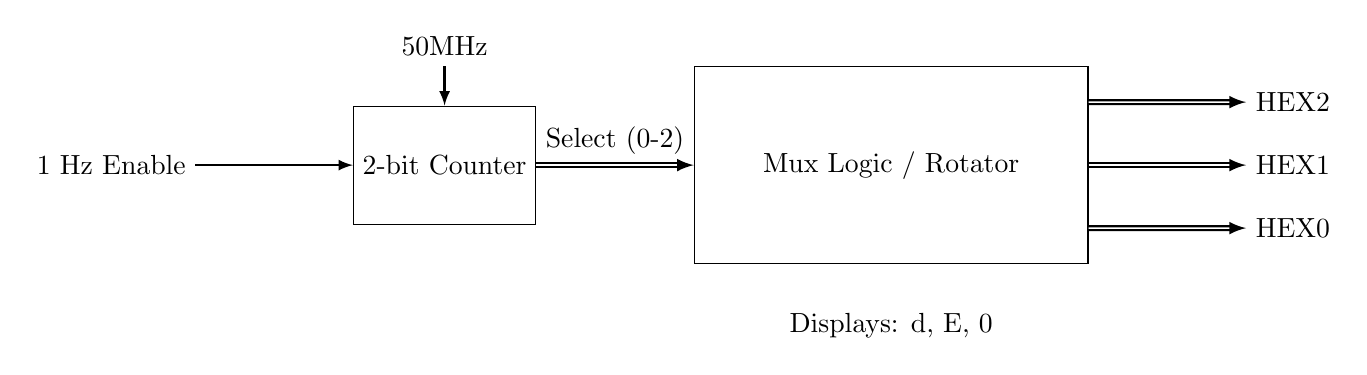
\begin{tikzpicture}[auto, node distance=2cm,>=latex]
    % Counter
    \node [draw, minimum width=2cm, minimum height=1.5cm] (cnt) {2-bit Counter};
    \node [left=of cnt] (clk) {1 Hz Enable};
    \draw [->, thick] (clk) -- (cnt.west);
    
    \draw [<-, thick] (cnt.north) -- ++(0, 0.5) node[above] {50MHz};
    
    % Logic / Muxes
    \node [draw, minimum width=5cm, minimum height=2.5cm, right=2cm of cnt] (mux) {Mux Logic / Rotator};
    
    % Connections
    \draw [->, thick, double] (cnt.east) -- (mux.west) node[midway, above] {Select (0-2)};
    
    % Outputs
    \node [right=of mux, yshift=0.8cm] (hex2) {HEX2};
    \node [right=of mux] (hex1) {HEX1};
    \node [right=of mux, yshift=-0.8cm] (hex0) {HEX0};
    
    \draw [->, thick, double] (mux.east) ++(0, 0.8) -- (hex2);
    \draw [->, thick, double] (mux.east) -- (hex1);
    \draw [->, thick, double] (mux.east) ++(0, -0.8) -- (hex0);
    
    % Text
    \node [below=0.5cm of mux] {Displays: d, E, 0};

\end{tikzpicture}

    \caption{Block diagram for rotating word.}
    \label{fig:rotate_small}
\end{figure}

A block diagram corresponding to this circuit is shown in Figure \ref{fig:rotate_small}.

There are many ways to design the required circuit. One solution is to re-use the VHDL code designed in Laboratory Exercise 1, Part V. Using that code, the main change needed is to replace the two switches that were used to select the characters being rotated on the displays with a 2-bit counter that increments at one-second intervals. Note that the counter for this circuit must also use the 50-MHz clock signal.

For reference, an example of a 2-bit wide 4-to-1 multiplexer is shown in Figure \ref{fig:mux_4to1}.

\begin{figure}[H]
    \centering
    \begin{minted}[frame=single, fontsize=\small, linenos]{vhdl}
LIBRARY ieee;
USE ieee.std_logic_1164.all;

ENTITY mux_2bit_4to1 IS
    PORT ( S : IN STD_LOGIC_VECTOR(1 DOWNTO 0);
           U, V, W, X : IN STD_LOGIC_VECTOR(1 DOWNTO 0);
           M : OUT STD_LOGIC_VECTOR(1 DOWNTO 0));
END mux_2bit_4to1;

ARCHITECTURE Behavior OF mux_2bit_4to1 IS
BEGIN
    PROCESS ( S, U, V, W, X )
    BEGIN
        CASE S IS
            WHEN "00" => M <= U;
            WHEN "01" => M <= V;
            WHEN "10" => M <= W;
            WHEN "11" => M <= X;
            WHEN OTHERS => M <= (OTHERS => '0');
        END CASE;
    END PROCESS;
END Behavior;
    \end{minted}
    \caption{A 2-bit wide 4-to-1 multiplexer.}
    \label{fig:mux_4to1}
\end{figure}

For reference, an example of a decoder that outputs "d", "E", "0", and blank space is shown in Figure \ref{fig:decoder_de0}.

\begin{figure}[H]
    \centering
    \begin{minted}[frame=single, fontsize=\small, linenos]{vhdl}
LIBRARY ieee;
USE ieee.std_logic_1164.all;

ENTITY hex7seg IS
    PORT ( hex : IN STD_LOGIC_VECTOR(1 DOWNTO 0);
           display : OUT STD_LOGIC_VECTOR(0 TO 6));
END hex7seg;

ARCHITECTURE Behavior OF hex7seg IS
BEGIN
    PROCESS ( hex )
    BEGIN
        CASE hex IS
            WHEN "00" => display <= "1000010"; -- d
            WHEN "01" => display <= "0110000"; -- E
            WHEN "10" => display <= "0000001"; -- 0
            WHEN OTHERS => display <= "1111111"; -- Blank
        END CASE;
    END PROCESS;
END Behavior;
    \end{minted}
    \caption{A decoder for d, E, 0, and blank.}
    \label{fig:decoder_de0}
\end{figure}

\section*{Part VI}

Augment your circuit from Part V so that it can rotate the word "dE0" over all 6 7-segment displays on your DE0-CV board (HEX5-0). The shifting pattern is shown in Table \ref{tab:rotate_large_pattern}. Similar to Part V, the counter for this circuit must also use the 50-MHz clock signal.

\begin{table}[H]
    \centering
    \begin{tabular}{|c|c|c|c|c|c|c|}
    \hline
    Clock Cycle & HEX5 & HEX4 & HEX3 & HEX2 & HEX1 & HEX0 \\
    \hline
    0 &   &   &   & d & E & 0 \\
    1 &   &   & d & E & 0 &   \\
    2 &   & d & E & 0 &   &   \\
    3 & d & E & 0 &   &   &   \\
    4 & E & 0 &   &   &   & d \\
    5 & 0 &   &   &   & d & E \\
    \hline
    \end{tabular}
    \caption{Rotating the word dE0 on six displays.}
    \label{tab:rotate_large_pattern}
\end{table}

\begin{figure}[H]
    \centering
    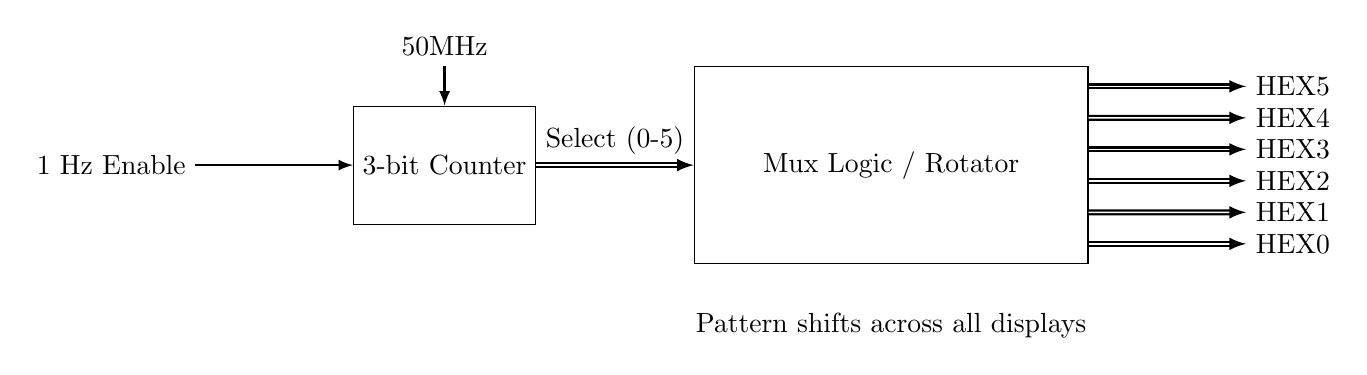
\begin{tikzpicture}[auto, node distance=2cm,>=latex]
    % Counter
    \node [draw, minimum width=2cm, minimum height=1.5cm] (cnt) {3-bit Counter};
    \node [left=of cnt] (clk) {1 Hz Enable};
    \draw [->, thick] (clk) -- (cnt.west);
    
    \draw [<-, thick] (cnt.north) -- ++(0, 0.5) node[above] {50MHz};
    
    % Logic / Muxes
    \node [draw, minimum width=5cm, minimum height=2.5cm, right=2cm of cnt] (mux) {Mux Logic / Rotator};
    
    % Connections
    \draw [->, thick, double] (cnt.east) -- (mux.west) node[midway, above] {Select (0-5)};
    
    % Outputs
    \node [right=of mux, yshift=1.0cm] (hex5) {HEX5};
    \node [right=of mux, yshift=0.6cm] (hex4) {HEX4};
    \node [right=of mux, yshift=0.2cm] (hex3) {HEX3};
    \node [right=of mux, yshift=-0.2cm] (hex2) {HEX2};
    \node [right=of mux, yshift=-0.6cm] (hex1) {HEX1};
    \node [right=of mux, yshift=-1.0cm] (hex0) {HEX0};
    
    \draw [->, thick, double] (mux.east) ++(0, 1.0) -- (hex5);
    \draw [->, thick, double] (mux.east) ++(0, 0.6) -- (hex4);
    \draw [->, thick, double] (mux.east) ++(0, 0.2) -- (hex3);
    \draw [->, thick, double] (mux.east) ++(0, -0.2) -- (hex2);
    \draw [->, thick, double] (mux.east) ++(0, -0.6) -- (hex1);
    \draw [->, thick, double] (mux.east) ++(0, -1.0) -- (hex0);
    
    \node [below=0.5cm of mux] {Pattern shifts across all displays};

\end{tikzpicture}

    \caption{Rotating the word over all displays.}
    \label{fig:rotate_large}
\end{figure}

The block diagram for rotating the word across all displays is shown in Figure \ref{fig:rotate_large}.

Implement the circuit and demonstrate its operation on the DE0-CV board.

\vspace{1cm}
\noindent \textbf{Updated By:} R. Sutthaweekul \\
\textbf{Release Date:} 2026-01-02

\end{document}
